\documentclass[13pt]{article}
\usepackage{amsmath}
\usepackage{amssymb}
\usepackage{amsthm}
\usepackage{color}
\usepackage{graphicx}
\title{A phylogenetic and population genetic model of protein evolution}
\author{}
\begin{document}
\maketitle
%%%%%%%%%%%%%%%%%%%%%%%%%%%%%%%%%%%%%%%%%%%%%%%%%%%%%%%%
\section{Introduction/Abstract}
Empirical and mechanistic models of amino acid replacement have been constructed to explain protein evolution since 1978 (Dayhoff et al). Yang et al. (1998) implemented a few mechanistic models at the level of codons and explicitly model the biological processes involved, including different mutation rates between nucleotides, translation of the codon triplet into an amino acid, and the acceptance or rejection of the amino acid due to selective pressure on the protein. We present a new codon model for protein evolution that can 1) empirically estimate the weighting factors for the Grantham matrix of amino acid similarities and use simulations and information from empirical data to find cases where populations of intermediate size may evolve faster than populations of large size.\\

\textit{Brief description of classical empirical and mechanistic models, the motivation of the new model.}
%%%%%%%%%%%%%%%%%%%%%%%%%%%%%%%%%%%%%%%%%%%%%%%%%%%%%%%%
\section{Model}
Our model works for homologous protein-coding sequence without gaps or with gaps removed. We use a continuous time Markov process to model substitutions among the amino acids within a protein-coding sequence. The states of the Markov process are the 20 natural amino acids (nonnatural amino acids can be easily added), and we use a $20 \times 20$ rate matrix $Q=(Q_{ij})$ where $Q_{ij}$ represents the instantaneous rate that amino acid $i$ will be substituted by amino acid $j$. As usual the row sum of $(Q_{ij})$ equals $0$ and $P(t) = \exp (tQ)$, where $P_{ij}(t)$ is the probability that amino acid $j$ replaces $i$ after time $t$. \\

We assume that mutations occur on the codon level at the three codon positions independently. Therefore, more than one nucleotide substitutions are not allowed to occur instantaneously as mutations involving more than one position during time $\Delta t$ will have probabilities $\Delta t^2$ and should be ignored. Based on the $4 \times 4$ mutation rate matrix for nucleotides the mutation rates $\mu_{ij}$ among 20 amino acids are calculated.

Consider a protein as a sequence of amino acid, assume that there is an optimal amino acid for each position. Any non-optimal amino acid at a position is subjected to selection, the strength of which depends on the physiochemical distance (Grantham, Science 1974) between the observed and optimal amino acids and magnitude of the selection force. \\

Suppose a protein of length $n$ has a sequence of optimal amino acids $\hat{\mathbf{a}} = (\hat{a}_1, \hat{a}_2, \cdots \hat{a}_n)$  and the observed sequence of amino acids is $\mathbf{a} = (a_1, a_2, \cdots, a_n)$. At position $k$, the selection coefficient is $s_k$ and let $\mathbf{s}=(s_1,s_2,\cdots,s_n)$. The overall physiochemical difference (distance) $d$ between amino acids $i$ and $j$ consist of 3 components: $D_{ij} = [\alpha (c_i-c_j)^2 + \beta (p_i - p_j)^2 + \gamma (v_i - v_j)^2]$, where $c, p$ and $v$ represent composition, polarity and molecular volume, and $\alpha, \beta, \gamma$ are the corresponding weights for each component. The values for properties in amino acid difference formula is given by Grantham (1974). \\

Given the distance vector $\mathbf{d} = (d_1, d_2, \cdots, d_n)$ from the optimal protein and the selection strength $\mathbf{s}$, the functionality of a protein $\mathbf{a}$ with $n$ amino acids is defined as

%{\color{blue} Could the functionality function be changed in a better way?}\\
\begin{equation}
%F(\mathbf{a}|\hat{\mathbf{a}},\mathbf{s})= \prod_{k=1}^{n}e^{-d(a_k, \hat{a}_k)s_k}=e^{-\mathbf{d(\mathbf{a},\hat{\mathbf{a}})}\cdot\mathbf{s}}
%\label{eq:ftny}
%\end{equation}
%or other candidates:
%\begin{eqnarray}
%F(\mathbf{a}) & = & \prod_{k=1}^n \frac{1}{1+d_ks_k}\\
F(\mathbf{a}| \hat{\mathbf{a}},\mathbf{s})  =  \frac{n}{\displaystyle  \sum_{k=1}^n{(1+d_ks_k)}} \label{eq:harmonic}\\
%F(\mathbf{a}) & = & \frac{n}{\sum_{k=1}^{n}\frac{1}{e^{-d(a_k, \hat{a}_k)s_k}}}
%\end{eqnarray}
\end{equation}
The condition $\hat{\mathbf{a}},\mathbf{s}$ will be omitted from now on if there is no potential confusion.\\

%fixation probability 
The fixation probability of a single protein mutant $\mathbf{a}_j$ from a diploid population with wild type $\mathbf{a}_i$ is 
\begin{equation}
\pi_{ij} = \pi(\mathbf{a}_i \rightarrow \mathbf{a}_j ) = \frac{1-f(\mathbf{a}_i)/f(\mathbf{a}_j)}{1-(f(\mathbf{a}_i)/f(\mathbf{a}_j))^{2N_e}} = \frac{1-f_i/f_j}{1-(f_i/f_j)^{2N_e}}
\label{eq:fixation}
\end{equation}
according to Sella-Hirsh (Add reference)
where $f(\mathbf{a}_i)$ and $f(\mathbf{a}_j)$ are the fitnesses of $\mathbf{a}_i$ and $\mathbf{a}_j$. This is an approximation to the canonical formula 

\begin{equation}
\pi(\mathbf{a}_i \rightarrow \mathbf{a}_j,p) = \frac{1-e^{-2N_e ps}}{1-e^{-2N_es}}
\label{eq:fixcanonical}
\end{equation}

\noindent where $p$ is the initial frequency of the mutant, and $s=(f_j-f_i)/f_i$ is the selection advantage of $\mathbf{a}_j$ comparing to $\mathbf{a}_i$ (note here $s$  is different from the selection strength defined above on the distance from optimal protein).
When there is a single mutant in the population, i.e. $p=1/(2N_e)$, the formula becomes
$(1-e^{-s})/(1-e^{-2N_es})$. Both formulae are valid under the same condition: $s, \frac{1}{N}, Ns^2 \ll 1$.\\


 
As in Gilchrist 2007, fitness of a protein is proportional to a function of cost, functionality and some scaling factors:
\[f(\mathbf{a}) \propto \exp\{-\frac{C\Phi q}{F(\mathbf{a})}\}\]
where $C$ is the expected cost of producing a single complete protein, $q$ is the scaling constant (seconds per ATP) determining the relationship between the rate of ATP usage and fitness $f$, and $\Phi$ is a measure of gene expression, specifically protein production rate (protein per second). \\

Combining $C\Phi q$ as one constant $A$, we have
\[ f(\mathbf{a}) \propto \exp\{-\frac{A}{F(\mathbf{a})}\} \]
%{\color{blue} Is the fitness function modifiable?}\\

In either S-H formula or the canonical formula of the fixation probability, the value that is of concern is $f_i/f_j$.
%\begin{eqnarray}
%\frac{f(\mathbf{a}_i)}{f(\mathbf{a}_j)} & = & \frac{f_i}{f_j} (\text{consider $C$ as constant for now}) \nonumber\\
%& = & \exp\Big[-\frac{A}{F(\mathbf{a}_i)} + \frac{A}{F(\mathbf{a}_j )}\Big] \nonumber\\
%& = & \exp \Big[-A\Big( \frac{1}{F(\mathbf{a}_i )} - \frac{1}{F(\mathbf{a}_j )}\Big)\Big] \nonumber\\
%& = & \exp \Big[-\frac{A}{\prod_{l\neq k}^n \exp(-d_l s_l)}\Big(\frac{1}{\exp(-d_k^i s_k)}-\frac{1}{\exp(-d_k^j s_k)}\Big)\Big]\nonumber\\
%& = & \exp\Big[ -\frac{A}{F_S}\Big(\exp(d_k^i s_k) - \exp(d_k^j s_k)\Big)\Big]
%\label{eq:fitnessratio}
%\end{eqnarray}
%where $d_k^i$ is the distance between the amino acids at position $k$ in $\mathbf{a}_i$ and $\hat{\mathbf{a}}$ , which is the only position where $\mathbf{a}_i$ and $\mathbf{a}_j$ differ. $F_S$ is the part of functionality shared by sites of the 2 proteins except site $k$. \\
If the functionality is defined as in Equation \ref{eq:harmonic}, we have the following:

\begin{equation}
\frac{f(\mathbf{a}_i)}{f(\mathbf{a}_j)} = \prod_{k=1}^n\Big( \frac{f(\mathbf{a}_i^k)}{f(\mathbf{a}_j^k)}\Big)^{\frac{1}{n}}
\end{equation}


i.e. the fitness ratio of the whole protein is the geometric mean of the fitness ratios between the two proteins for all sites. Therefore, when $\mathbf{a}_i$ and $\mathbf{a}_j$ only differ at position $k$, it becomes  
\[\frac{f(\mathbf{a}_i)}{f(\mathbf{a}_j)} = \Big( \frac{f(\mathbf{a}_i^k)}{f(\mathbf{a}_j^k)}\Big)^{\frac{1}{n}}\]
and
\begin{eqnarray}
\frac{f(\mathbf{a}_i)}{f(\mathbf{a}_j)} & = &\exp \Big[-A\Big( \frac{1}{F(\mathbf{a}_i )} - \frac{1}{F(\mathbf{a}_j )}\Big)\Big] \nonumber\\
& = & \exp\Big[ -\frac{A}{n}(d_k^i s_k - d_k^j s_k)\Big]\\
& = & \exp\Big[ -\frac{C\Phi q}{n}(d_k^i s_k - d_k^j s_k)\Big]\\
& = & \exp\Big[ -\frac{C\Phi q s_k}{n}(d_k^i - d_k^j)\Big]
\end{eqnarray}
\noindent
this quantity is only related to site $k$. It is easy to see that all the sites are independent in the sense that if there are more than 1 site that differ, the ratio is simply a product of ratios at all sites. Therefore we will focus on proteins with only one amino acid site, i.e. a single amino acid.\\
%and is independent of all other sites. Therefore, the sites are independent. In this case, the parameters $C, \Phi, q$ and $s_k$ are all multiplied together, only $C$ depends on $n$, so they should be treated as a composite parameter, as inseparable. \\
%{\it Should we relax the condition so that the mutation between proteins with more than 1 different position is also possible?}\\

We assume that the mutation rate $\mu$ between 2 proteins that differ at more than one position is 0. Instantaneous substitution rate from $\mathbf{a}_i$ to $\mathbf{a}_j$ is the product of mutation rate and fixation rate:
\begin{equation}
u_{ij} = 2N_e \mu_{ij} \pi_{ij}
\label{eq:subrate}
\end{equation}

where $\mu_{ij}$ is the mutation rate from $\mathbf{a}_i$ to $\mathbf{a}_j$, and $\mu_{ij} = 0$ when more than 1 position differ in the codons that code for $\mathbf{a}_i$ and $\mathbf{a}_j$ Note that the mutation and fixation are both at amino acid level. \\

With the values for $(s, \alpha, \beta, \gamma, C, \Phi, q, N_e)$, we can find the $20 \times 20$ instantaneous rate matrix $Q$ and have the Markov process set up. Then we can calculate the likelihood given the sequence data on the tips of a phylogenetic tree $T$ with topology and branch lengths given, therefore to find the maximum likelihood estimates for parameters. \\

Identifiability --- Since $C, \Phi, q$ and $s$ are multiplied together as a composite parameter, we fix the values of $C, \Phi, q$ and search for MLE for $s$. For the weights of 3 components in the amino acid distance formula, if they are multiplied by a same constant, the likelihood will not be affected. So we will fix $\alpha$ and look for the MLEs for $\beta, \gamma$ as only the relative ratios are identifiable. Suppose that the tree is given, there are $3$ parameters that we are estimating here: $s, \beta/\alpha$, and $\gamma/\alpha$.



\section{Results}
\subsection{Model accuracy}
To access the model accuracy, we first simulate data using different parameter values, find the MLEs for the parameters from the simulated data, and then investigate the accuracy of the estimates by looking at the mean squared error and confidence intervals.\\

We did simulation with number of sites $100, 500, 1000$, $s = 0, 0.01, 0.1$, under 6 different trees, including 2 with 4 tips, 2 with 8 tips and 2 with 16 tips. 



\begin{center}
\line(1,0){250}
\end{center}

To check if the simulation is done correctly, here are some results. For simplicity, only 3 states (amino acids) are considered now. \\

1. Check that the way to do simple simulation and to find the stationary probability is correct.\\

Given the instantaneous substitution rate matrix $W$ for a Markov process with stationary probability vector $\mathbf{p}$ , $\mathbf{p}$ can be calculated by taking any row of the matrix $\exp(Wt)$ where $t$ is big enough to guarantee that the process has already reached stationarity. \\

On the other hand, if $W$ comes from the mutation and fixation processes, then $\mathbf{p}$ can also be found by S-H's formula of stationary probabilities
\begin{equation}
\frac{p_i}{p_j} = (\frac{f_i}{f_j})^{\nu} = \frac{W_{ji}}{W_{ij}}
\label{eq:stationary}
\end{equation}




Comparing $\mathbf{p}$ calculated in both ways verifies that S-H's formula is accurate. Next we compare $\mathbf{p}$ calculated from the simulation with that from either of the formulae. The way I found $\mathbf{p}$ is as follows:\\
\begin{enumerate}
\item Do simulations with long enough time so that there are at least $10,000$ substitutions in the simulated chain.
\item Cut off the first 100 observations, before the time when the process reaches stationarity.
\item Find the average time $\bar{t}$ taken for a certain number of substitutions (for example, 10), and record the state of the chain when the amount $\bar{t}$ of time passed.
\item Find the frequency of the observed states, hence the approximation of $\mathbf{p}$.
\end{enumerate}

\begin{center}
\line(1,0){250}
\end{center}

Following are some results.\\
\begin{enumerate}
\item Let $W$ be the substitution rate matrix between all the protein with 2 sites. Since there are only 3 states for each site, total number of protein is 9. Hence the dimension of the matrix $W$ is $9\times 9$.\\
\begin{figure}[here]
\centering
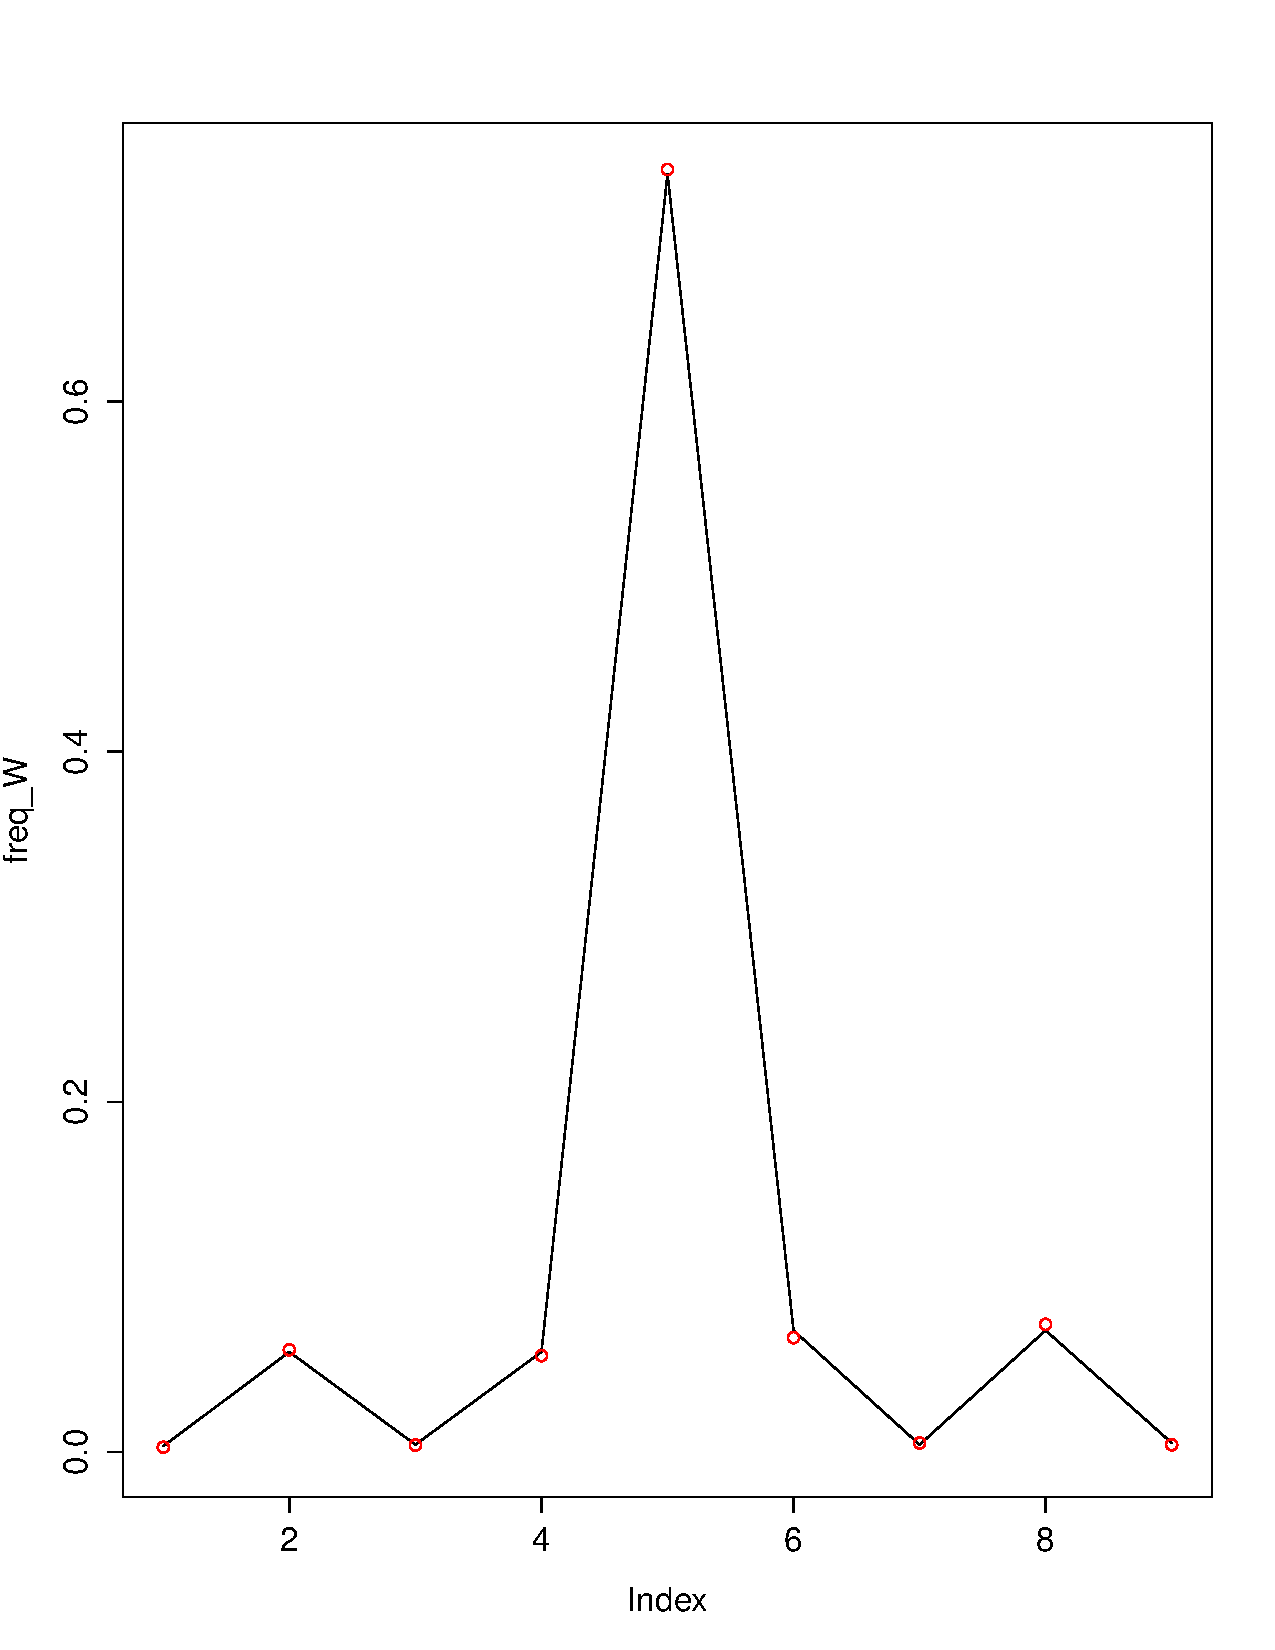
\includegraphics[scale=0.2]{freq_simple_sim.pdf}
\caption{Stationary probabilities with 2 sites}
\label{fig:freq2sites}
\end{figure}

In Figure~\ref{fig:freq2sites} on page ~\pageref{fig:freq2sites} the solid line connects the values of stationary probabilities for each state from theoretical calculation, and the red circles from simulation. \\
%Obviously the simulation is done correctly and analyzed correctly in this case.\\

\item Another simulation is done with 2 sites (3 states for each site) for each protein, starting with $(1,2)$, with optimal protein $(2,2)$, selection coefficient  0.1, running time $10^9$, sites dependent. The stationary probabilities are:
\begin{table}[here]
\begin{center}
\begin{tabular}{rrrrrrrrrr}
  \hline
  1 & 2 & 3 & 4 & 5 & 6 & 7 & 8 & 9 \\ 
  \hline
 0.003364677 & 0.057514946 & 0.004235888 & 0.058025656 & 0.727881756 & 0.069636795 & 0.004130742 & 0.070132484 & 0.005077057 \\ 
0.003324449 & 0.057134781 & 0.004132447 & 0.057134781 & 0.730153540 & 0.069429813 & 0.004132447 & 0.069429813 & 0.005127929 \\ 
   \hline
\end{tabular}
\end{center}
\end{table}

First row is from simulation, second row is from Sella-Hirsh's formula. They are very close to each other. The number of steps in this simulation is $669061$, which is relatively big.\\

\item A simulation with 3 sites and 3 states for each site confirmed the correctness of simulation. The chain starts with $(1,1,1)$, with optimal protein $(2,2,2)$, selection coefficient $0.01$, running time $10^8$, sites dependent. The number of observations is $216126$. Figure~\ref{fig:freq3sites} on page ~\pageref{fig:freq3sites} is a plot of stationary probabilities from both simulations and Sella-Hirsh's formula.
\begin{figure}[here]
\centering
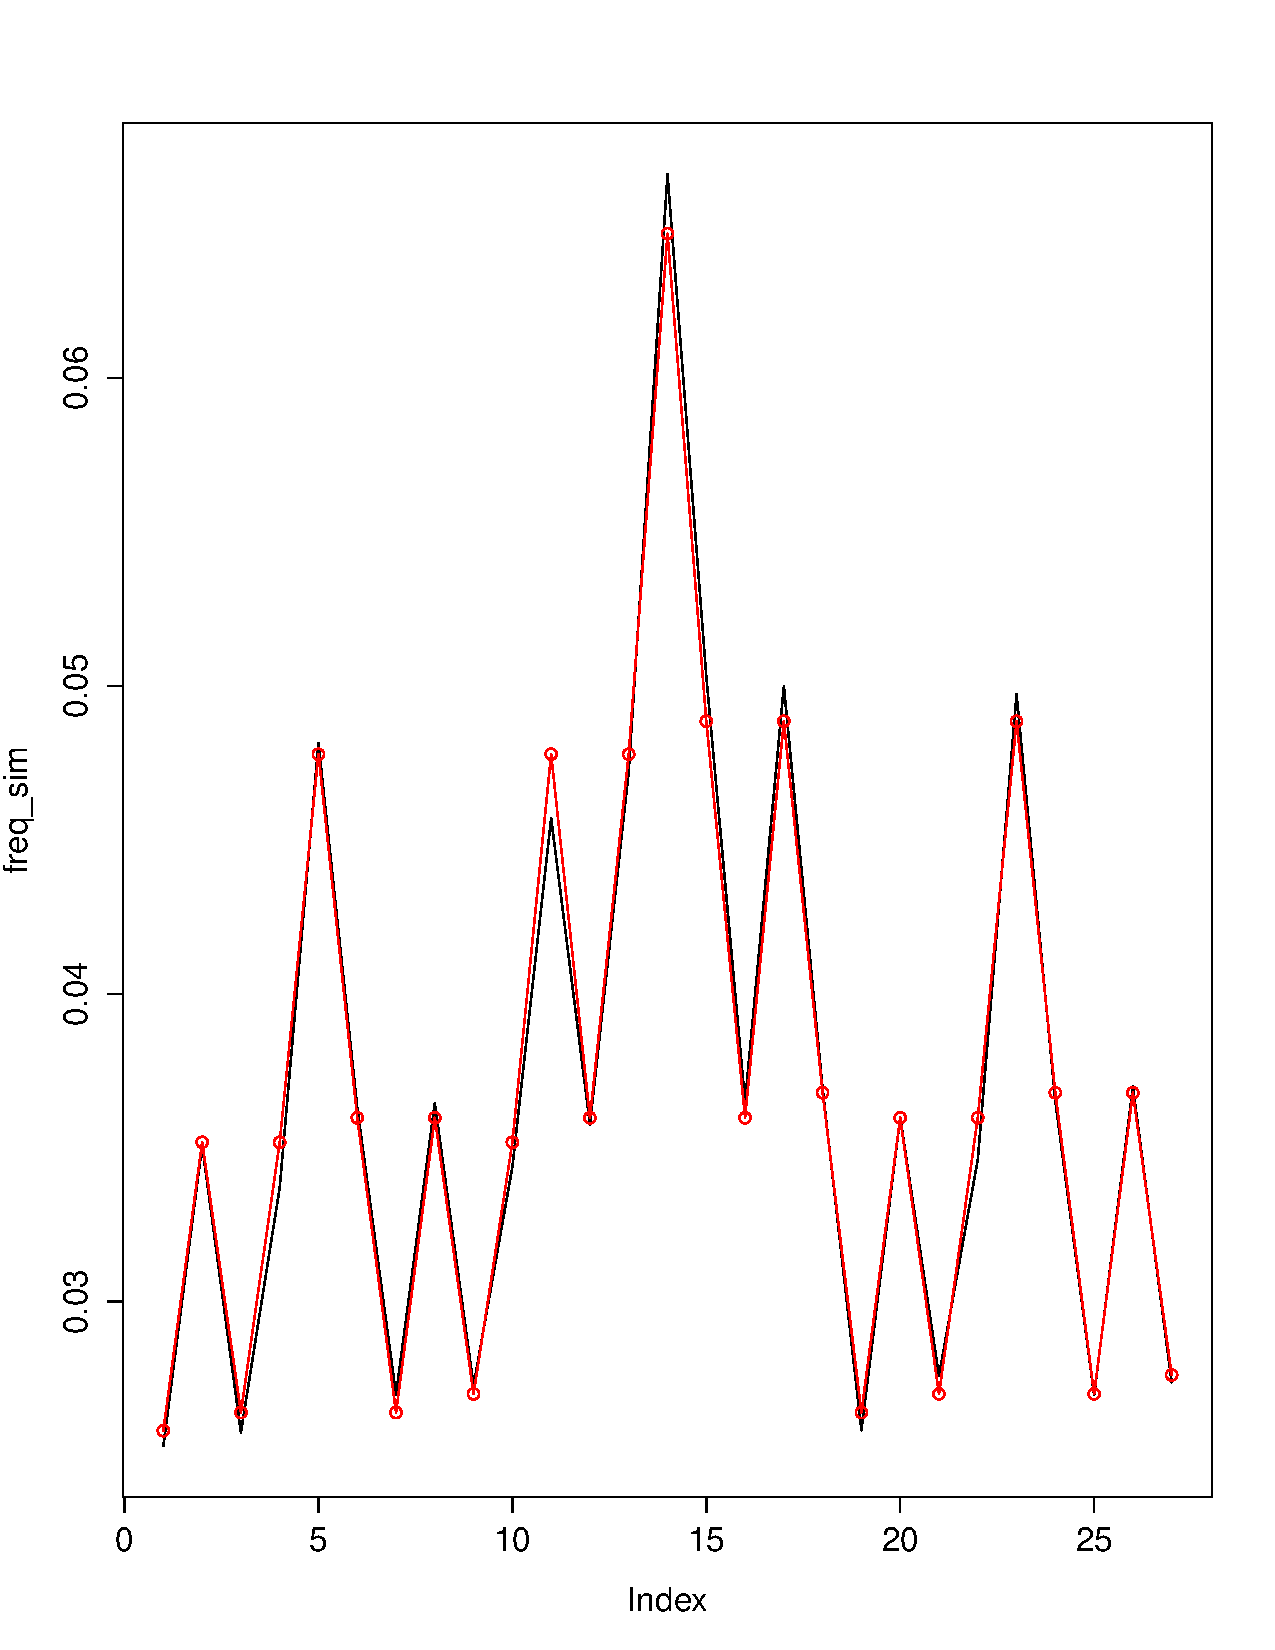
\includegraphics[scale=0.3]{3sites3states.pdf}
\caption{stationary probabilities with 3 sites}
\label{fig:freq3sites}
\end{figure}

\end{enumerate}

\begin{center}
\line(1,0){250}
\end{center}

Questions to answer next:
\begin{enumerate}
\item How to construct phylogeny from the simulated data?\\

\item How to approximate the functionality (and other variables of concern) in the site-dependent case using site-independent case?\\

In site-independent case, it's equivalent to assuming that every other site is at the optimal amino acid hence the functionality at those sites is 1. When the process has reached stationarity, if $\Phi$ is high and selection is strong, then the frequency of optimal amino acids will be high hence the assumption is reasonable. However, when $\Phi$ is small or selection is very weak, there tend to be more non-optimal amino acids at many sites.\\

Consider the case when there are only 2 sites (amino acids) in the protein, fix the second site at a certain amino acid and let only site 1 change. How does site 2 affect the stationary distribution at site 1?\\

From \eqref{eq:fitnessratio},
\begin{equation}
f_{ij} = \frac{f_i}{f_j} = \exp\Big(-\frac{A}{F_2}(e^{d_is_1} - e^{d_js_1})\Big)
\label{eq:fitratioindep}
\end{equation}
In site-independent case, we assume site 2 is at the optimal amino acid, i.e. $F_2 = 1$, therefore
\begin{equation}
f_{ij}^{\text{ind}} = \exp\Big(-A(e^{d_is_1} - e^{d_js_1})\Big)
\end{equation}

The relationship between the two fitness ratios is
\begin{equation}
f_{ij}^{\text{ind}} = (f_{ij})^{F_2}
\end{equation}

If site 2 is not at the optimal amino acid, then $F_2 < 1$. Now consider the fitness ratios between an amino acid ($aa_i$) and the optimal amino acid ($aa_o$).\\
\begin{eqnarray}
f_{io} & = & \exp\Big(-\frac{A}{F_2}(e^{d_is_1} - 1)\Big)\\
f_{io}^{\text{ind}} & = & (f_{io})^{F_2}
\end{eqnarray}
Since $f_{io} < 1$, $f_{io}^{\text{ind}} > f_{io}$, the fixation probability from an arbitraty amino acid to the optimal amino acid is higher in the site-dependent case. In other words, the selection strength at one site is {\bf higher} when other sites are not at the optimal amino acids.\\

Let's see what happens with stationary distributions under site-independent and -dependent cases. From \eqref{eq:stationary}, 
\begin{equation}
\frac{p_i}{p_o} = \big(\frac{f_i}{f_o}\big)^\nu = (f_{io})^\nu
\end{equation}
Therefore 
\begin{equation}
(\frac{p_i}{p_o})^{\text{ind}} = (f_{io}^{\text{ind}})^\nu = (\frac{p_i}{p_o})^{F_2} > \frac{p_i}{p_o}
\end{equation}

This result could easily be generalized when the functionality $F_S$ is known for othere sites and only one site is changing, with $F_2$ replaced by $F_S$. Simulations also verified the relation.\\

Rewriting the equation \eqref{eq:fitnessratio}, we can see
\begin{equation}
\frac{f_i}{f_j} = \exp\Big[-A\Big(e^{d_k^i s_k - \ln F_S} - e^{d_k^j s_k -  \ln F_S}\Big)\Big]
\end{equation}
What does this reflect the effect of $F_S$ on selection strength at site $k$?\\

The most essential and what we are most interested in are the fixation rates from one protein to another, under both site-dependent and site-independent cases. If this is clear, the substitution rates and stationary distribution will follow, also the mean fitnesses. On the other hand, fixation probability is a function of fitness ratio, which also determines the stationary probabilities.\\

Now we already know how to express the fitness ratio in site-dependent case in terms of that in site-independent case, with functionality at other sites as exponent, when there is only one site that is different between two proteins. \\

To get the fitness ratio between any two proteins, we could use proteins that are one site away from them as bridges and represent the ratio as a product of several ratios we already know. For example:

\begin{eqnarray*}
\frac{f_{AA}}{f_{BB}} & = & \frac{f_{AA}}{f_{AB}} \cdot \frac{f_{AB}}{f_{BB}}\\
\frac{f_{AA}}{f_{AB}} & = &(\frac{f^2_A}{f^2_B})^{-F_A}\\
\frac{f_{AB}}{f_{BB}} & = &(\frac{f^1_A}{f^1_B})^{-F_B}
\end{eqnarray*}

If furthermore, the selection coefficients at the first and second positions are the same, then $\frac{f^2_A}{f^2_B} = \frac{f^1_A}{f^1_B} = \frac{f_A}{f_B}$ in site-independent case. Therefore
\begin{equation*}
\frac{f_{AA}}{f_{BB}} = (\frac{f_A}{f_B})^{-F_A-F_B}
\end{equation*}

If there are more than 2 sites that are different, then there need to be more than one intermediate proteins to relate them together. For example,
\begin{equation*}
\frac{f_{AAA}}{f_{BBB}} = \Big(\frac{f_A}{f_B}\Big)^{-F_{AA}-F_{AB}-F_{BB}}
\end{equation*}
However, if the selection coefficients are not the same across the sites, this relationship does not hold any more. The reason is that even fitness ratio in site-independent case depends on the selection coefficient at that particular site. 
\end{enumerate}
%Next step: set the mutation rate to be a different number, add mutation bias, move from amino acid level to codon level.

\begin{center}
\line(1,0){250}
\end{center}

Parameters to investigate during the optimization (optimx):\\
\begin{enumerate}
\item $s, \Phi, C, q, N_e$, some of them are correlated to each other and cannot be split separately
\item tree topologies (at different extremes), branch lengths, number of tips
\item ancestral sequences --- stationary, uniform, same sequence as used in the simulation
\end{enumerate}

Hessian matrix, variance, information; confidence interval, bootstrapping; ...

\begin{center}
\line(1,0){250}
\end{center}

Meeting on Thursday, Mar 8, 1012.
\begin{enumerate}
\item Do the plots of MLE bias with respect to number of sites (200, 400, 800 or more in between) : first, fix other parameters, estimate $s$; second, estimate $\Phi$ while fix other parameters. Do this for trees with 4 tips and 8 tips.
\item Estimate the composite parameter.
\item Instead of giving the equilibrium frequencies, make it depend on the parameters as from Sella-Hirsh's formula, and do the optimization that way.
\item Let $s$ vary according to Gamma distribution instead of being fixed, and estimate the Gamma parameter(s).
\end{enumerate}

Profiling R code:

> Rprof(file="rprof.out")
> R command
> Rprof(NULL)

under unix, use command:
R CMD Rprof rprof.out
\end{document}
